\section{Input / Output}

Every OS has an I/O subsystem, which handles all interaction between the machine and the outside world. The I/O subsystem abstracts individual hardware devices to present a more or less uniform interface, provides a way to name I/O devices, schedules I/O operations and integrates them with the rest of the system, and contains the low-level code to interface with individual hardware devices. \medskip

To an OS programmer, a \textbf{device} is a piece of hardware visible from software. It typically occupies some location on a bus or I/O interconnect, and exposes a set of hardware registers which are either memory mapped or in I/O space. A device is also usually a source of interrupts, and may initiate Direct Memory Access (DMA) transfers. \medskip

The \textbf{device driver} for a particular device is the software in the OS which understands the specific register and descriptor formats, interrupt models, and internal state machines of a given device and abstracts this to the rest of the OS.


\subsection{Data Transfer}

\textbf {Programmed I/O} consists of causing input/output to occur by reading/writing data values to hardware registers. This is the simples form of communication. It is fully synchronous, so the CPU always has to be involved. Further it is polled, the device has no way to signal that new data is ready. \medskip

\textbf{Interrupts} can be used to signal the availability of new data and solve the polling problem. But the problem of CPU involvement still persists.
\begin{center}
	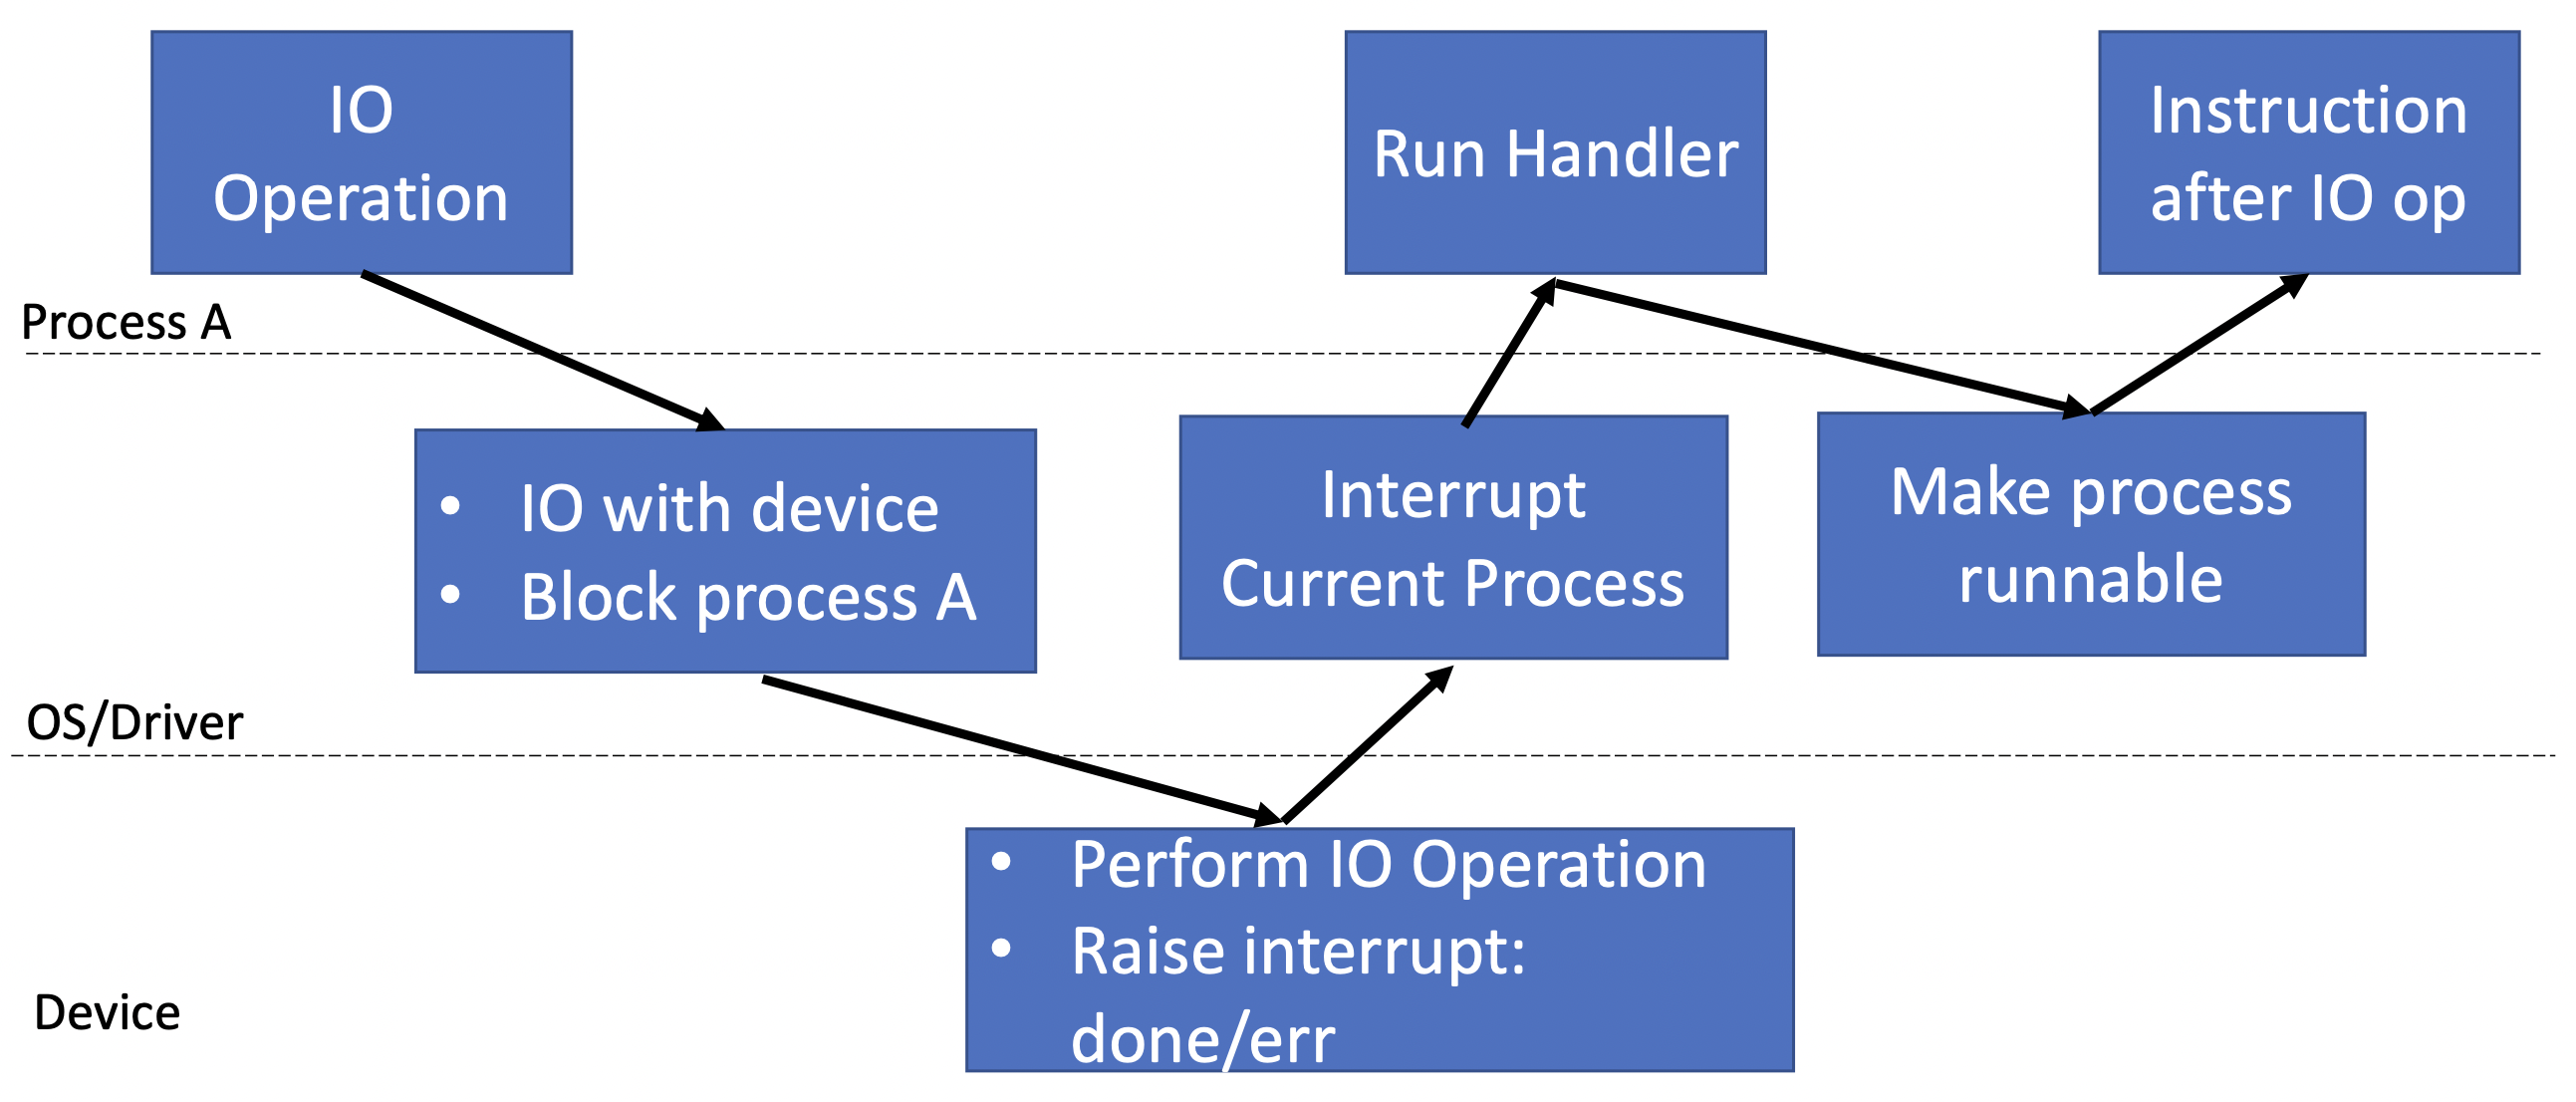
\includegraphics[width=\linewidth]{data_transfer_interrupt.png}
\end{center}

\textbf{Direct Memory Access} or DMA, a device can be given a pointer to buffers in main memory and transfer data to and from those buffers without further involvement from the CPU. A single interrupt is used to signal the end of data transfer. DMA is, for the most part, physical (not virtual) access to memory. Further DMA transfers to and from main memory may or may not be coherent with processor caches.


\subsection{Asynchrony}

Device drivers have to deal with the fundamentally asynchronous nature of I/O: the system must respond to unexpected I/O events, or to events which it knows are going to happen, but not when. \medskip

The \textbf{First-level Interrupt Service Routine} (FLISR) is the code that executes immediately as a result of the interrupt. It runs regardless of what else is happening in the kernel. As a result, it can't change much since the normal kernel invariants might not hold. \medskip

Since I/O is for the most part interrupt-driven, but data is transferred to and from processes which perform explicit operations to send and receive it. Consequently, data must be buffered between the process and the interrupt handler, and the two must somehow rendezvous to exchange data. There are three canonical solutions to this problem: \medskip

A \textbf{deferred procedure call}, is a program closure created by the 1st-level interrupt handler. It is run later by any convenient process, typically just before the kernel is exited. \medskip

A \textbf{driver thread}, sometimes called an interrupt handler thread, serves as an intermediary between ISR and processes. The thread starts blocked waiting for a signal either from the user process or the ISR. When an interrupt occurs or a user process issues a request, the thread is unblocked (this operation can be done inside an ISR) and it performs whatever I/O processing is necessary before going back to sleep. Driver threads are heavyweight: even if they only run in the kernel, the still require a stack and a context switch to and from them to perform any I/O requests. \medskip

The third alternative, is to have the FLISR convert the interrupt into a message to be sent to the driver process. This is conceptually similar to a DPC, but is even simpler: it simply directs the process to look at the device. However, it does require the FLISR to synthesize an IPC message, which might be expensive. In non-preemptive kernels which only process exceptions serially, however, this is not a problem, since the kernel does not need locks. \medskip

\textbf{Bottom-half handler} - the part of a device driver code which executes either in the interrupt context or as a result of the interrupt. \medskip

\textbf{Top-half handler} - the part of a device driver which is called "from above", i.e. from user or OS processes.


\subsection{Device Models}

The device model of an OS is the set of key abstractions that define how devices are represented to the rest of the system by their individual drivers. It includes the basic API to a device driver, but goes beyond this: it encompasses how devices are named throughout the system, and how their interconnections are represented as well. \medskip

\textbf{UNIX device model:}
\begin{itemize}
	\item Character Devices - used for unstructured I/O and present a byte-stream interface with no block boundaries.
	\item Block Devices - used for structured I/O and deal with blocks of data at a time.
	\item Network Devices - correspond to a network interface adapter. It is accessed through a rather different API.
	\item Pseudo Devices - a software service provided by the OS kernel which it is convenient to abstract as a device, even though it does not correspond a physical piece of hardware (e.g. \textit{/dev/random}).
\end{itemize}


\subsection{Protection}

Another function of the I/O subsystem is to perform protection. Ensuring that only authorized processes can access devices or services offered by the device driver and that a device can't be configured to do something harmful.\medskip

UNIX controls access to the drivers themselves by representing them as files, and thereby leveraging the protection model of the file system. DMA-capable devices are in principle capable of writing to physical memory anywhere in the system, and so it is important to check any addresses passed to them by the device driver. Even if you trust the driver, it has to make sure that it’s not going to ask the device to DMA somewhere it should not. One approach is to put a memory management unit (MMU) on the path between the device and main memory, in addition to each core having one.
